\documentclass[11pt,twoside]{article}

\usepackage{paperlighter}

% Recommended, but optional, packages for figures and better typesetting:
\usepackage{microtype}
\usepackage{graphicx}
\usepackage{subfigure}
\usepackage{booktabs} % for professional tables
\usepackage{titlesec}

\setcounter{secnumdepth}{4}

% Attempt to make hyperref and algorithmic work together better:
\newcommand{\theHalgorithm}{\arabic{algorithm}}


% For theorems and such
\usepackage{amsmath}
\usepackage{amssymb}
\usepackage{mathtools}
\usepackage{amsthm}

\usepackage[capitalize,noabbrev]{cleveref}

%%%%%%%%%%%%%%%%%%%%%%%%%%%%%%%%
% THEOREMS
%%%%%%%%%%%%%%%%%%%%%%%%%%%%%%%%
\theoremstyle{plain}
\newtheorem{theorem}{Theorem}[section]
\newtheorem{proposition}[theorem]{Proposition}
\newtheorem{lemma}[theorem]{Lemma}
\newtheorem{corollary}[theorem]{Corollary}
\theoremstyle{definition}
\newtheorem{definition}[theorem]{Definition}
\newtheorem{assumption}[theorem]{Assumption}
\theoremstyle{remark}
\newtheorem{remark}[theorem]{Remark}

% Todonotes is useful during development; simply uncomment the next line
%    and comment out the line below the next line to turn off comments
%\usepackage[disable,textsize=tiny]{todonotes}
\usepackage[textsize=tiny]{todonotes}



\slimtitle{Design Manual - F21DG}
\slimauthor{F21DG}


\begin{document}

\lightertitle{Design Manual - F21DG}

\lighterauthor{Callum Stewart, Saad Badshah, Abigail Rivera, Daniel Scott, Bruce Wilson, Sebastian Zebrowski}


\section{Preface}

\subsection{Introduction}

Contained within this report is a documentation of the testing strategy employed whilst developing this application. Thorough testing of system components, through both automated and manual techniques, has been utilized all along development to ensure the delivery of a robust, reliable software system that achieves the system requirements set forth in the Design Specification.

For the most part, this document is comprised of component level Unit Tests which verify that a given component works correctly with a mix of expected and unexpected behaviour patterns. Although it is hard, if not impossible, to anticipate every edge case that could occur, reasonable thought has been given towards likely behaviours that can be expected in day-to-day usage of the application. 

Unfortunately, Integration Testing had to be done manually by developers close to the end of the project's development cycle due to issues with testing frameworks and last-minute snags which required urgent attention to address. The steps taken within these manual Integration tests, are however, documented within this report. 

\subsection{Explanation of Testing Strategy}

As mentioned above, a combination of both manual \& automated testing was rigorously employed throughout the course of development to ensure the final deliverable was up-to-scratch and met the requirements outlined in the Design Specification.

To perform our automated testing for our JavaScript components, the {\bf\href{https://jestjs.io/}{Jest}} framework was employed. Jest is a unit-testing framework developed \& maintained by Meta (Facebook's parent organization), and as such came complete with extensive documentation and examples to reference from. Jest allows for configuration and tweaks to be made to it via an optional {\bf jest: \{...\}} parameter in a project's {\bf package.json} file. This came in especially useful when attempting to mock SessionStorage and DOMElement behaviours which, by default, aren't supported \& aren't trivial features to implement. 

Due to an unfamiliarity with the Jest framework, and the difficulty incurred when attempting to mock specific behaviours of Browser components and classes, there was an element of manual JavaScript testing involved as well. This manual testing was performed by writing out a series of objectives \& example inputs that a class would be expected to deal with and then simulating user behaviour to assess the robustness of the specific functionality being tested (i.e. Uploading Files). The console in the Browser would be monitored for print statements and any warnings/errors that were thrown in this process.

Because of an unfamiliarity with GitLab and time-pressure stemming from upcoming deadlines, a CI/CD pipeline was not established for this project, which in turn resulted in a requirement for the Python code to be manually tested without a framework. Elements of this testing strategy have been preserved under the {\bf tests\ } folder in the source code, specifically being used for generating .csv test data dynamically and then supplying it to the STFT logic to validate the analysis being performed.

\newpage
\section{End-User guide}
\subsection{Introduction}
This guide demonstrates how to use our developed application for time series decomposition.
Our demo video can be found at: 
\href{https://www.overleaf.com/learn}{Application Demonstration Video}

\subsection{Quick Start Guide}
This is a quick guide to help a user get started with our application.
\begin{figure}
\centering
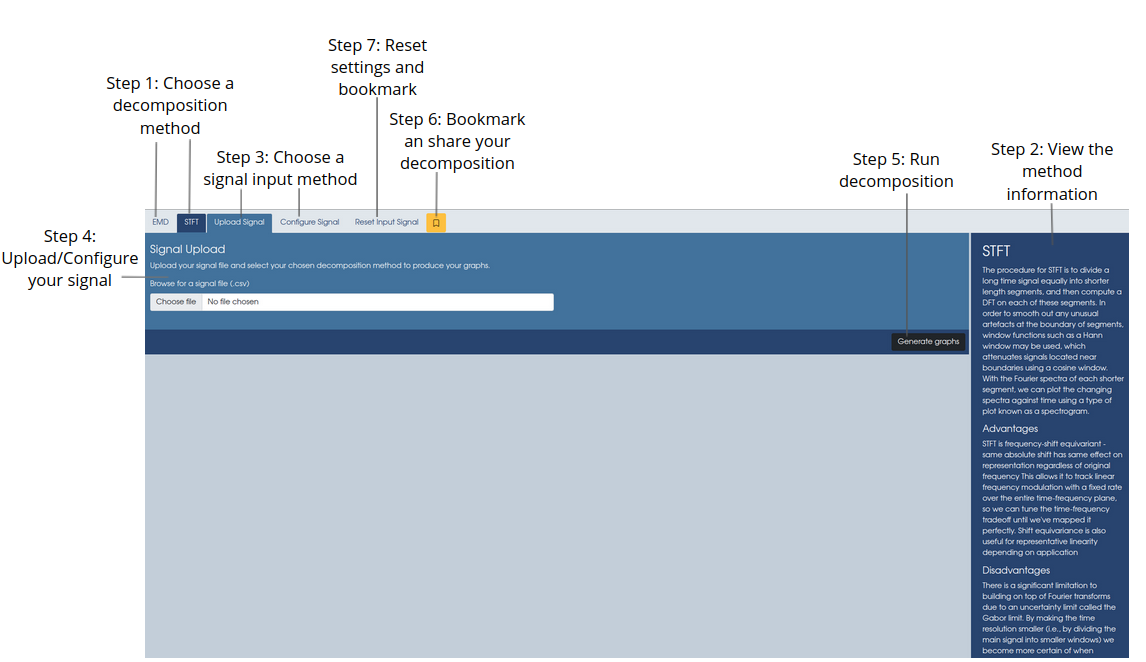
\includegraphics[width=1.0\textwidth]{img/quickguidesteps.png}
\caption{\label{fig:Application Interface}Application Interface}
\end{figure}


\subsection{User Instructions}
\subsubsection{Configuring a combined signal}
\begin{figure}
\centering
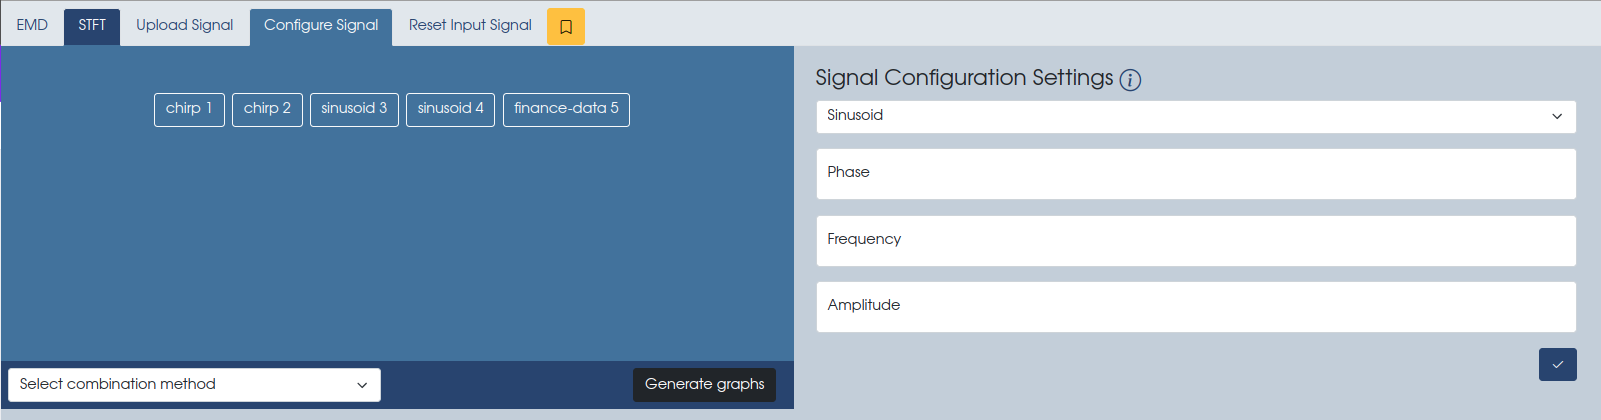
\includegraphics[width=1.0\textwidth]{img/signalconfig.png}
\caption{\label{fig:Signal Configuration}Signal Configuration}
\end{figure}

\begin{enumerate}
\item Click on the configure signal tab found on the top panel.
\item Select a signal type from the drop down in the 'Signal Configuration Settings' panel.
\item Input your values into the various fields.
\item Press the tick button to add your signal. Your signal should appear on the left hand panel.
\item To edit or delete your signal, click on the signal and make changes or delete in the 'Signal Configuration Settings' panel.
\item Set your combination method for your signals. Note: only sinusoids and trends should be combined using product method.
\end{enumerate}

\subsubsection{Uploading a signal}
\begin{figure}
\centering
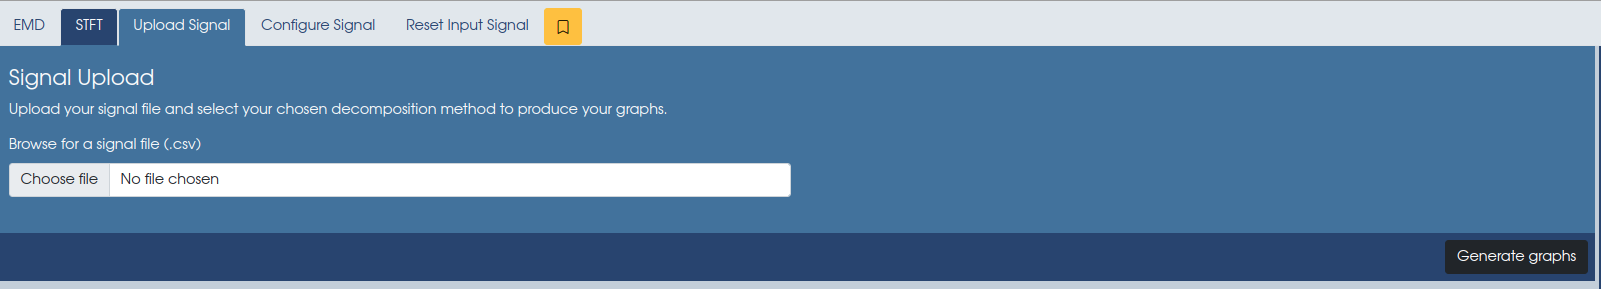
\includegraphics[width=1.0\textwidth]{img/signalupload.png}
\caption{\label{fig:Signal Upload}Signal Upload}
\end{figure}

\begin{enumerate}
\item Click on the upload signal tab found on the top panel.
\item Choose a file to upload. Note: Only .csv files are currently supported.
\item You should receive an upload complete message if the upload was a success.
\end{enumerate}

\subsubsection{Selecting decomposition method}
\begin{enumerate}
\item Click on either the 'EMD' or 'STFT' tab on the top panel to select a method. An information panel will open up on the right hand side.
\item EMD (Empirical Mode Decomposition): This method will result in various IMF (Intrinsic Mode Function) graphs and a Hibert-Huang Spectrum  
\item STFT: This method will result in an FFT (Fast Fourier Transform) graph and a resultant spectrogram.
\end{enumerate}

\subsubsection{Running decomposition method}
\begin{enumerate}
\item Once you have completed configuring your settings, click on 'Generate graphs'.
\item Your decomposition graphs should appear below the settings panel. This may take a couple of minutes based on your settings.
\item You may click on your charts on the left hand panel to expand them into the larger view area.
\end{enumerate}

\subsubsection{Bookmarking}
\begin{enumerate}
\item Once you have completed configuring your settings, simply click on the yellow bookmark button.
\item Your settings will be saved into your URL and your URL is now copied to your clipboard and can be pasted anywhere.
\item You should now be able to access your settings in a different window by pasting the URL into the address bar.
\end{enumerate}

\label{systemdesc}\section{System Description}

This section contains documentation detailing the top-level design of the system, alongside further documentation on how the future developer reading this
can modify and reuse this code in the future. It will first guide through an overview of how the entire system works, 
building up background information that should be understood first, then continuing on to dive into specifics.

\subsection{Design overview}

\subsubsection{Pyodide.}\label[]{pyodide}

That word may not mean much, however it is critical to how this whole project fits together. 
Pyodide is a full CPython reference implementation 
compiled and embedded entirely in browser using a virtual instruction set language named WebAssembly. Using WebAssembly, it is possible to get near (system, configuration, and more dependant)
native run-times of languages while encapsulating software systems in browser tabs. Even while being a relatively new 
technology - initially appearing in 2017 \cite{10.1145/3062341.3062363} - it 
is supported in the most commonly used browsers, including mobile OS browsers. 

Not only does this allow custom Python code that can be run directly in browser, but we can also make
use of Pythons humongous pre-existing library of pre-built packages (wheels) that are written in pure python. 

Note: Some packages do however contain C code alongside their Python code, but in most cases using the same system that enabled the CPython implementation to be compiled to WebAssembly,
we can do the same with the Python packages containing C, allowing almost any package to run entirely in browser.

In summary, Pyodide enables the use of pre-existing, tested, and verified packages for signal generation, EMD and STFT analysis, and graph generation, combining them carefully 
- alongside performing personalised unit and integration testing - into the software system. 
However Pyodide is not all we shall need to produce the full working system, and there are many caveats with Pyodide itself.


\subsubsection{How we make use of Pyodide.}\label[]{howweusepyodide}

Pyodide appears to be an all-powerful tool, however how much use can we really get out of it? While it is able to solve many problems
revolving around complex algorithm implementation, signal generation and combining, and graph generation, we still need methods using standard web technologies, i.e. HTML, CSS, JavaScript,
to make the system. It is these cross-overs between Pyodide technologies and standard web technologies that created the majority of challenges during implementation.

We made use of several Python packages during implementation to varying degrees, these packages are listed below:

\begin{itemize}\label[]{requiredpackages}
    \item {\bf NumPy - } NumPy is the fundamental Python package for scientific computing, implementing multidimensional arrays, matrix structures, alongside basic FFT's and signal generation techniques.
    We cover the specifics of which functions that we use in the \hyperref[signalgeneration]{Signal Generation}, \hyperref[emdsection]{EMD}, and \hyperref[stftsection]{STFT}.
    sections.

    \item {\bf SciPy - } SciPy is a scientific Python package built on-top of NumPy, incorporating further functions for signal processing, optimisation, and statistics. We make use of several available
    functions when \hyperref[signalgeneration]{Generating Signals}, alongside performing \hyperref[stftsection]{STFT Analysis}.

    \item {\bf mpld3 - }\label[]{mpld3} A Python package that exports a graph MatPlotLib plot to HTML, CSS, JavaScript, and most importantly D3. D3 is a powerful graphics 
    library for JavaScript, that allows for interactive graphs entirely in browser. More specifically, mpld3 makes use of a the MatPlotLib mplexporter framework, which parses an 
    input MatPlotLib plot, and outputs a JSON representation. This representation can then be read in by mpld3.js, a standalone JS framework built on-top of D3, which exports the HTML graph.
    We also directly use d3 when creating a spectrogram to display STFT analysis. This is because generating a full interactive spectrogram plot in mpld3 can be quite intensive and slow, whereas
    generating the spectrogram data and then displaying it interactively with d3 alone is significantly faster.

    \item {\bf micropip - } A Python package specifically for Pyodide, this package allows loading Python packages from PyPi or any arbitrary source at runtime. 

    \item {\bf emd - } A Python package for emperical mode decomposition and related spectral analyses. This package is used to deconstruct the supplied input signal, be that generated or uploaded, and return a list of
    IMF's to be displayed in line graphs to the user.

    % \item {\bf Pandas - } The Pandas Python package is used specifically for signal object representation in this system, however in general Pandas is a fast powerful and easy to use data analysis and manipulation tool.

\end{itemize}

The use of Pyodide also has impacts on how the rest of the system is shaped, and choices were made during development on how we would work around caveats that came to light during 
cross technology implementation. These caveats are detailed below, and may be referenced later in the manual:

\begin{itemize}
    \item {\bf Web Workers - } Using Pyodide with its default implementation runs all code in the main tab render thread. This can present a serious
    problem in any system that makes use of graphical interface, as during any long length computation, the tab can become completely unresponsive, harming the user experience.
    To fix this, we made use of Pyodide only inside Web Workers. These Web Workers are a simple means to run scripts in background threads, and therefor allow Python scripts to run
    in a completely separate thread, leaving the tab render thread to continue unimpaired. 
    There are however consequences of this fix. When Pyodide is constructed in a Web Worker, it creates its entire own interpreter. This means we cannot
    make use of the Python global namespace for information handling or sharing, and must share messages from Web Workers back to the Javascript storage handler via post messages.
    Further complicating the matter, there are restrictions imposed by both Pyodide and Javascript on what objects can be passed and auto-translated between environments.
    We are able to alleviate this problem though, by passing around Javascript objects that execute the Python code and only returning the final result - using the bullet point below - 
    a raw HTML graph, with all included controls and data, at no point does there require any Python $ \to $ Javascript object translation.
    A final problem is that the page DOM nor session storage can be accessed from inside a Web Worker Pyodide interpreter, and any attempt to access parts of the `js' package causes Pyodide to crash.
    However as we return values from the Web Workers, there is no need to access the DOM directly, and this does not present a problem.

    \item {\bf MatPlotLib - } MatPlotLib is a comprehensive Python package used to create various forms of visualisation. In this case, and as detailed later in the 
    \hyperref[stftsection]{specific details on STFT implementation} and \hyperref[emdsection]{specific details on EMD implementation}, we make use of the spectrogram
    and line graph visualisations contained within the library. However, when using the Web Worker technology detailed above, MatPlotLib makes an attempt to access part of the `js' package
    as part of its loading process. This immediately crashes the Web Worker thread, even when we don't want MatPlotLib to access the DOM directly, just create a graph to be stored.
    It can however, be fixed. MatPlotLib makes use of a frontend $ \leftrightarrow $ backend system,  with the frontend handling
    the user facing code, and the backend handling the heavy lifting behind-the-scenes to make the figure. MatPlotLib also automatically selects which backend to use depending on the available
    system, and we found that is part of the default backend code that is attempting to access the `js' package. 
    To stop this, we can force MatPlotLib to use a different backend, such as AGG (exports high quality images using the Anti-Grain Geometry engine), enabling graphs to be saved as required.

    \item {\bf mpld3 - } While MatPlotLib can generate graph images and interactive graphs when using a framework such as Qt, without these frameworks it cannot alone export interactive graphs
    like those that we need to display the signals. We use mpld3 to generate these interactive graphs from inside Python. However, the same issue was encountered with this library as detailed above in the
    MatPlotLib package - it was trying to access the `js' package inside a Web Worker. Once again to solve this, we changed the backend that mpld3 used, which prevented the problem.

    \item {\bf emd - } While STFT functionality was baked into SciPy, we had to find another package capable of performing EMD analysis. In theory, this was easy, as the `emd' package on PyPi - a large Python package repository - 
    had the `py3-none-any' tag. This meant that the wheel had no particular abi restrictions, and could be used on any platform - in general this meant that inside the package there was only pure Python code, and no C source code.
    This was needed, as mentioned in the \hyperref[pyodide]{Pyodide Description}, as any wheel with pure Python code could be run in Pyodide with no modification, where as a wheel containing C code would need to be compiled separately.
    However, `emd''s dependencies did not contain only pure Python code. Following the chain, `emd' required `sparse', which implemented n-dimensional sparse arrays, but again was all Python code. `sparse' then required `numba', which was a 
    just-in-time (JIT) compiler for numerical functions in Python. This is where the problem lay, as this JIT compiler made use of `LLVMLite' a lightweight python binding for writing JIT compilers, 
    which made use of `LLVM', a collection of reusable compilers and toolchains. Attempting the compilation of `LLVMLite' to WebAssembly ourselves, and then searching through troves of online information, we found that through our own
    attempts, and the attempts of numerous other users, that this process would prove incredibly difficult.

    We decided to start back at the drawing board instead, and delve into the `emd' package code, and find where the `sparse' package was being used. We found that the only place that it was being used, was for further spectral
    analysis than was required in the scope of this project. So as such, we decided to strip out the requirement for `sparse', and repackage the whole `emd' library and distribute it directly via our
    system (allowed under the license GPLv2+).

    \item {\bf Hilbert-Huang Transform (HHT) - } To perform the additional HHT and produce a resulting spectrogram, a custom script was made contained in \verb|FILLINNAMEHERE|, which makes use of the HHT code inside `SciPy'.
    \todo[]{We might need to remove this if we dont implement it}

    \item {\bf JSON Bottleneck - } While making use of JSON means that we do not face any problems with object type auto-translation between Python and JavaScript, it was found during testing that this serialisation and deserialisation
    to and from JSON is a considerable bottle neck in the speed of the system, especially considering that whole arrays of thousands of samples from time-series are being converted. If performance was more of a focus of this application,
    and more time was at hand, this problem could be avoided using the provided `JsProxy' and `PyProxy' objects, however as performance was not a focus, this has been left for future developers to implement if desired.

    \item {\bf Bookmarking - } As mentioned previously, due to the use of Web Workers, the Python global name space for storing Python generated signal types is not available. However, 
    we can work around this by using the browsers local session storage as a replacement, simply involving writing JavaScript handling code.
\end{itemize}


\subsubsection{How Pyodide fits in with the rest of the system.}

Hopefully now through the previous sections it is clear that while Pyodide has some hurdles that must be jumped, it provides an excellent staging ground for this system to launch from.
It must now integrate with the rest of the client side web stack, being executed for example through JavaScript events from button presses, or returning data through post messages to be added
to the page DOM.

To keep things simple, we have a single Web Worker running Pyodide inside, setup importing the required packages, and implementing any fixes to the caveats in the system as detailed \hyperref[howweusepyodide]{above}.
This single Web Worker is setup to accept and return post messages, a method of communication between threads in JavaScript. An initial JSON post message is sent to the Worker with signal information (stored
in session storage) and analysis type. This JSON message is then forwarded into the Pyodide code, where Python decides which method of analysis should be performed, generates the signals from input parameters,
combines said signals, and finally performs the analysis. The result of all this Python code is a string of HTML code, that is returned once more through a post message from the Web Worker to the main thread,
where it is injected into the DOM.

This remaining web stack makes use of Bootstrap material design to provide a consistent and modern design to the front end, detailed further in the \hyperref[frontendsection]{Front-end interface section}.
Pyodide graphs are then generated in HTML and injected directly into the DOM, making use of the \hyperref[mpld3]{mpld3 package}. Alongside this, the whole system only uses plain JavaScript for simplicities sake.

\subsection{Front-end Interface}\label[]{frontendsection}

The front-end interface is built so that any user can experiment and perform EMD and STFT analysis both on their own uploaded data and on data that they have generated through this system.

The bulk of the front-end is contained with in the \verb|src/index.html| file. Inside the \verb|<head>| of the document, the styled version of bootstrap is loaded, alongside our bundled \verb|main.bundle.js| 
JavaScript code. The system makes use of webpack to bundle all JavaScript code into a single file, alongside optimising and removing any duplication. In the remainder of the \verb|<body>| of the document, 
bootstrap's buttons and navigation constructs are used to create the navigation bar, along with option buttons. Further in the document, the modal containing information on the types of signal that 
the user can generate is created. This is created using an accordion class from bootstrap, allowing for a drop-down menu for each signal type. Inside these signal types, details on the available
input parameters are also listed, providing clear information to the user on what their choice of input signals will achieve. 

Moving on to the \verb|main.js| file, the first step is loading in all JavaScript modules and their relevant functions into the \verb|main.js| file. Using this module and loading system means modularity can
be implemented during development, making code easier to understand, test, and refactor, while using \verb|webpack| as mentioned previously to bundle our code together when it is served to the end user.
Next, document \verb|querySelector|'s are used to find, and then attach click event listeners to the required user-interface buttons. Using this method means as much arbitrary code as required can be
executed upon button press, such as saving bookmarks or setting the signal analysis method.
Alongside this, the \verb|DOMContentLoaded| event is attached to. This event is only called when the page has completed loading, and means that it is possible to manipulate the DOM in any way required,
creating a \verb|promise| that the page is ready.
Once this promise is fulfilled, previously mentioned module classes are instantiated, such as \verb|InfoPanel|. These classes expose functions that generate or modify content in the DOM. In the example 
of \verb|InfoPanel|, the \verb|displayInfoPanel| function is exposed, taking a boolean argument on whether it should be displayed or not. This class and function also grab data from a separate JSON
file named \verb|methodInfo.json|. When required to be displayed, the relevant information from the \verb|methodInfo.json| file is displayed to the user, providing advantages, disadvantages, and a description
of each signal analysis type.

\subsubsection{Input Selection}
The input selection is shown as two different tabs on the front end namely 'Upload Signal' and 'Create Signal'. These two different tabs are implemented through modules \verb|UploadSignal.js| and \verb|ConfigureSignal.js|. 
Uploading signals is mainly covered through the fileIO module for file processing and passing through the signal data as the front-end simply includes the file input element and the button to generate the 
graphs as there are no other configuration settings involved with this method other than choosing the analysis method.
Configuring signals within the application is implemented through dynamic forms created for each of the signal types as they all required different parameters to create. 
These are loaded in through HTML templates using the ES6 syntax and create a button or 'chip' for every signal produced so they can be edited and deleted as necessary. 
These actions all update the URL as required to ensure it is accurate when the user bookmarks the application state. All the form text inputs have been limited to numerical values though the required attribute has not been able to be implemented as there were issues with Bootstrap custom forms and using browser defaults. 
There is also a help link on the signal form to give more information on the signal types units. The combination method selector includes a tool-tip to explain that combining via product should be limited to certain data types as it was decided that we should not restrict the user experimentation as much as possible. 

\subsubsection{Bookmarking}
As part of our original specification we were tasked to create a method of saving and sharing the users application settings and signal configurations. The implemented solution is based off creating a bookmark 
feature that copies the current URL to the user's clipboard. Bookmarking is handled within the \verb|bookmark.js| module and is used to update the URL parameters with the users settings and choices through the UI.
 In order to consistently update the URL when an analysis method is chosen or signal parameter is added or edited the URL is updated on each button click which triggers a UI change for that action as well as saving the URL string within session storage. 
 This string can then be processed to create an object that can be used as the input data for the graphs. There are different methods for dealing with the signal parameters as the keys follow a format of \verb|[signal number]-[signal parameter name]=[signal value]| in order to differentiate and identify the different signal's values within the URL.

\subsection{File IO}

\subsubsection{Main Logic}
The application supports users supplying their own input data for both EMD and STFT analysis. 

This functionality is achieved in a separate class in the source code located at {\bf src/fileIO.js}. 

The constants required by the class, and those that reference it, are declared at the beginning. These include an array of supported file types (this is currently just {\bf .csv}, but utilizing an array will make it easier in the future to add more supported file-types) and a {\bf csvDataKey}, which is used as the key to store uploaded csv data in the browser's sessionStorage.

In typical use-cases, the class is invoked via the {\bf parseFile()} method, which will attempt to read a .csv file selected by the user. There is a safety check to verify that a file has indeed been selected by the user, and the {\it 'Generate Graphs'} button hasn't just been pressed without something to process: if that is the case, the method will safely return early, without an error.

After verifying that a file has indeed been selected by the user, there is another safety check to validate that the type of file selected is supported; this is in addition to specifying this as a parameter of the HTML input option in {\bf src/modules/uploadSignal.js}. If more file types are to be supported in the future, this parameter should reference the static {\it supportedFileTypes} array mentioned earlier to reduce tediousness of the work, as only one file will need to be altered to allow for more file extensions to be accepted.
If, for some reason, a file-type has slipped through the cracks and this check fails, an alert will be displayed informing the user that the given file-type is not supported, and to try again. The method will then return early.

Finally, just before the file is read in, there is a check to determine whether {\it csvDataKey} in browser storage is currently populated; if it is, then it means it's data from a previous upload and should be cleared before progressing. 

Afterwards, a new {\bf FileReader()} object is created to read in the supplied file. Error/Progress/Abort/Load handlers are all attached to the object to ensure robustness. Once the {\it 'loadend'} event is triggered, a call is made to the {\bf loaded(target) function}. This is the function responsible for actually parsing the data read in by the file reader.

Upon being called, the {\it loadend} method will change the status displayed to the user as "Finished Loading!" and will then call the {\bf csvToArray} method to convert the text which has just been read in to a JavaScript array. Once finished being converted, the resultant array is then converted into a JSON string and stored in sessionStorage under the {\it csvDataKey} key. The object is converted to a JSON String to preserve the structure of the data (without this, the '[' and ']' are lost, making the data much harder to parse) and for consistency with other classes utilizing sessionStorage.

The {\bf csvToArray} method invokes an external library called {\it convertCSVToArray} which handles all the transformation logic. The headers are stripped, the output type is supplied as 'array' and the separator is designated as ',', and the library handles the rest. Once the data is read in, there is a check to ensure that only numerical data exists in the resultant array via the {\bf onlyNumericalDataInCSVArray(arr)} method.

The {\bf onlyNumericalDataInCSVArray} method iterates through the entire array to ensure that there is no non-numerical data contained in the array (this is to make things easier for the Python code down the line). The only exception to this is if the code represents 'e', 'E' or '-' in place of {\it exponent} values. If this check fails, the method returns false and an error is thrown in the parent {\bf csvToArray} method. Otherwise, the method returns true. 

After this process is completed, the data contained in the supplied file is available to be read by any class that requires it via the {\it csvDataKey} key in the browser's sessionStorage. 

\subsubsection{Helper Class}
A small class was created to assist with reading and writing to the Browser's sessionStorage. This class is located in {\bf src/helpers/sessionStorage.js}.

A disclaimer is at the top of the class notifying which browser versions support session storage (and thus the functionality to upload files). The remainder of the class is then populated with getter/setter methods as well as a method to check if a value is associated with a given key. 

\subsubsection{CSV File Format}
This section provides guidance for how to structure your .csv file(s) so that they can be read by the application. 

Although the title of your headers doesn't particularly matter, their number and ordering does. The application expects your headers to follow the convention {\bf Time, Value}, such that the first value represents the time of the event (your X axis value), and the second represents the value at the given time (your Y axis value). 

An example is provided below: 
\begin{table}[!ht]
    \centering
    \begin{tabular}{|l|l|}
    \hline
        {\bf Time} & {\bf Value} \\ \hline
        0.0 & 0.0 \\ \hline
        0.00628947 & 0.00012583 \\ \hline
        0.01257895 & 0.00050233 \\ \hline
    \end{tabular}
\end{table}


\subsection{Generating Graphs}\label[]{gengraphs}

The process of generating graphs, generating signals, combining signals, and performing analysis, is all performed in one large swoop, involving heavy use of Pyodide and Python,
and is subsequently outlined in the following section.

Prior to the journey beginning, when the page is initially constructed an instance of the Pyodide Web Worker must first be created. This Web Worker creates a Pyodide Python interpreter inside it, and installs the 
\hyperref[requiredpackages]{Required Packages}, using both micropip and the \verb|pyodide.loadPackage| methods. Once these packages have been loaded, and the Worker is satisfied that it is ready to receive data, it assigns a 
positive value to the \verb|pyodideReady| boolean, signalling to the rest of the code that the Worker is ready.

The Web Worker then sits idle, until the pressing of the \verb|Generate Graphs| button present in the \hyperref[frontendsection]{User Interface}. This button press calls an event, which in turn makes a chain of function calls.
First, it calls the \verb|displayLoadingGraphs| function contained inside the \verb|graphs.js| file. 
This function creates the placeholders for the graphs in the DOM, and adds a loading animation to the placeholders to tell the user that there is some background processing occurring.

Next, the \verb|handleCallPyodide| function from \verb|pyodideHelpers.js| is called, which creates in turns calls the \verb|evaluatePython| function, while creating a promise on said function to return some data for
future processing.
This \verb|evaluatePython| function creates a promise, which when resolved correctly, sends a post message to the previously mentioned Pyodide Web Worker containing the method that the data was created (uploaded or generated 
using the system), the analysis method to be performed, and if the signal was generated using the system, the information about the signal. The Web Worker then takes these input parameters, and decides which functions need to be called.
Error handling is baked into this process too, ensuring that the Web Worker is ready to receive data, with data verification taking place ensuring that the session storage is collected and passed through correctly.

If the signal provided was generated using the tool, then the \hyperref[signalgeneration]{Signal Generation} code shall be called, otherwise, the program will skip straight to the \hyperref[stftsection]{STFT} or \hyperref[emdsection]{EMD}
code.

\subsubsection{Signal Generation}\label[]{signalgeneration}

Signal generation is handled entirely in Python, inside the Pyodide Web Worker's \verb|script.py| file, with the signal data from the user passed in via the \verb|analysis_runner| or \verb|FUNCTIONNAMEHERE| function call. 
\todo[]{THIS NEEDS CHECKED, \\ may change depending on implementation}

One of these functions then parses the input data, and generates
signals according to the input parameters from the user, calling the relevant functions inside the \verb|signals.py| file. Inside this file, a separate function, e.g. \verb|simple_sin|, \verb|chirp|, \verb|white_noise|, is created, that 
accepts the required input parameters, and returns a time series of points over a predefined period. These functions also make use of the \hyperref[requiredpackages]{Required Packages}, specifically NumPy and SciPy, to generate
the time-series. Using these separate functions again introduces modularity, and allows modifying and testing of specific components.

\subsubsection{Signal Combining}

Signal combining is performed in a separate function to signal generation, with each of the initial generated signals from the user selected signals being passed in through a 2D array.
These signals are then combined depending on the selected combine type, either sum or product. Both of these functions are almost identical, however a $ + $ or $ * $ is used depending if the selected method is sum or product respectively.


\subsubsection{STFT Analysis}\label[]{stftsection}

STFT analysis is performed on either user uploaded data or tool generated signals depending on the choice made in the user interface. 
Either way, the process is the same, where the exposed \verb|FUNCTIONNAMEHERE| function is called, passing in the required input parameters (be that a combined signal from the tool, or user uploaded data).
\todo[]{CHECK FUNCTION NAME}

This function then returns a number of variables back to the caller. Previously this function made use of the same mpld3 method used in EMD analysis, however the spectrograph implementation was taking too long to generate,
and was outputting in too low a resolution. Instead of this, the raw JSON representing a spectrogram is output, and returned through the chain of calls, from \verb|stft_analysis| $ \to $ Web Worker $ \to $ post message 
$ \to $ \verb|evaluatePython| promise $ \to $ \verb|handleCallPyodide| promise callback. Inside this promise callback, the spectrogram data is then parsed, and fed into the d3 library directly. A custom graph generation JavaScript file 
contained within \verb|JAVASCRIPTFILEFORD3| is then used, which quickly generates a spectrogram, and replaces the placeholder graphs with this generated spectrogram.

Alongside this spectrogram data, along the same chain the combined signal graph and component signal graphs are also returned from the mpld3 library. These graphs we still generate using mpld3 as line graphs are fast, and still of high
quality, when generated using MatPlotLib.
\todo[]{THIS NEEDS CHECKED, AND MAY CHANGE}


\subsubsection{EMD Analysis}\label[]{emdsection}

EMD analysis is again performed on either user uploaded data or tool generated signals depending on the choice made in the user interface.
The process either way is the same, where the exposed \verb|analysis_runner| function is called, passing in the required input parameters (be that a combined signal from the tool, or user uploaded data).
\todo[]{CHECK FUNCTION NAME}

This function then returns a number of variables back to the caller. As EMD analysis returns a list of IMF's for viewing purposes, these graphs can be generated as line graphs over a common time base in mpld3, as line
graphs are quick to generate, and their HTML code can be returned through a series of calls. This chain flows as so: from \verb|emd_analysis| $ \to $ Web Worker $ \to $ post message 
$ \to $ \verb|evaluatePython| promise $ \to $ \verb|handleCallPyodide| promise callback. Inside this callback, the HTML graphs are parsed, and placed in the appropriate positions according to the placeholder graphs.

Alongside these IMF graphs, along the same chain the combined signal graph and component signal graphs are also returned from the mpld3 library. These graphs we still generate using mpld3 as line graphs are fast, and still of high
quality, when generated using MatPlotLib.
\todo[]{THIS NEEDS CHECKED, AND MAY CHANGE}

\section{Installation}


\section{Maintenance}


To keep the over-time functionality of the application without any unexpected crashes, the application should be maintained throughout its lifetime. 
To do the maintenance we will need to check up on the various packages and tools used in the implementation of the application to make sure that the features used at the time of the development of 
the application are still supported by the new and more updated packages and libraries. The main libraries that needs to be maintained for this web application are mentioned below
\subsection{Pyodide}

Pyodide is the backbone of this web application, all of the code is interlinked using pyodide and the libraries used in this application are converted to Web Assembly using Pyodide. 
The maintenance of Pyodide is the most important to do. To ensure the packages chosen during the development are still compatible with Pyodide will be checked by testing all the key functionalities 
of the packages that are used by pyodide to ensure the application runs smoothly and to ensure that dependencies for packages that we use all work and if they contain C code, are compiled to web assembly appropriately.
The Pyodide website will be checked to see if the modules are still supported or not, as pyodide updates their users on their website of the latest changes to the supported modules. 
Pyodide will be updated accordingly to ensure everything is working and to improve security risks.

\subsection{Graphing}
Another important feature of this web application is to have graphing features for the users to interact with. 
The libraries used for graphing such as d3, mpld3, and MatPlotLib will be also checked for any newer versions, specially d3 as it keeps getting updated versions, some of the code written in an older version might not 
be supported on the newer version, so its important to keep the version of d3 to be the one that supports the code written during development.
\subsection{General checks and updates}
Some of the other libraries used in the application such as node will be updates regularly to ensure the latest and updated security and performance. 
Ensuring long term compatibility with web assembly in case browsers add a permission - similar to the microphone permission - will also be looked out for to avoid any unexpected bugs.
\section{Troubleshooting}
This section will explain any known issues and how to fix them.

\begin{enumerate}
\item Browser not supported: Our application has been tested using Chromium Browsers, specifically Chrome v87 & v99. Incompatabilities were experienced with Firefox (specifically Firefox 78.15.0esr) and Safari (all versions), hence those browsers are not recommended for use. 
\item File not supported: Only .csv/.CSV files are supported. We recommend that you follow the format specified in the FileIO Section: E.g.  
Time,Value
0.0,0.0
0.00628947,0.00012583
0.01257895,0.00050233
... 
\end{enumerate}



\bibliographystyle{plainnat}
\bibliography{ref}

% \newpage
% \appendix
% \input{content/appendix}

\end{document}